\subsection{Получение информации о команде утилитой man}

\subparagraph{1) Что нужно было сделать?}

Получить информацию по командам ls и cd с помощью утилиты man. Изучить структуру man-документа.

\subparagraph{2) Как это сделали?}

\begin{MyVerbatimCode}[label=Debian terminal]
pavel-innokentevich-galanin@aspire-one-725:~$ man ls
\end{MyVerbatimCode}

Результат выполнения команды на~рисунке~\ref{fig:man} (стр.~\pageref{fig:man}).

\begin{figure}[!htp]
    \centering
    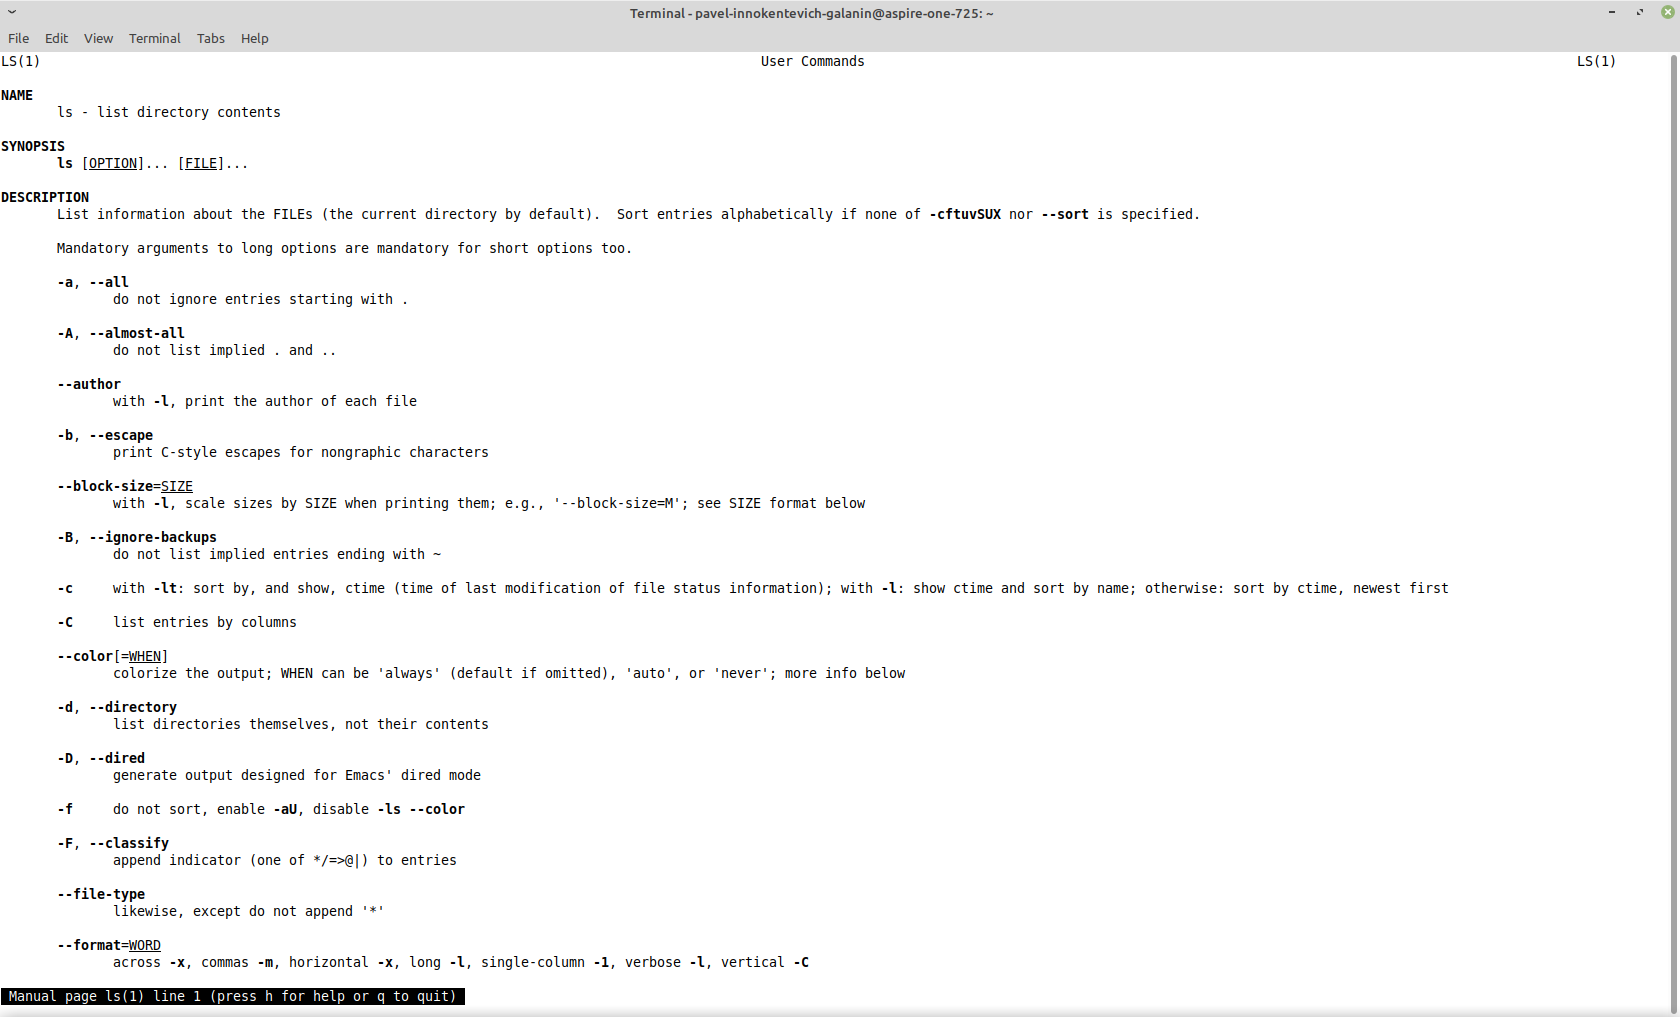
\includegraphics[width=11cm]
        {../input/task-1/5/man.png}
    \caption{man ls}
    \label{fig:man}
\end{figure}

\begin{MyVerbatimCode}[label=Debian terminal]
pavel-innokentevich-galanin@aspire-one-725:~$ man cd
No manual entry for cd
\end{MyVerbatimCode}

\subparagraph{3) Что получилось?}

Получили в консоль справочный файл о команде. Если справки нет, то выводится сообщение об отсутсвии.
